\documentclass[12pt,a4paper]{article}

\usepackage{graphicx}
\usepackage[margin=2.4cm]{geometry}
\usepackage{fontspec}
\usepackage{xeCJK}
\usepackage{xcolor}
\usepackage{booktabs}
\usepackage{hyperref}
\usepackage{array}
\usepackage{fancyhdr}

\setmainfont{Helvetica Neue}
\setsansfont{Helvetica Neue}
\setCJKmainfont{Hiragino Sans GB}
\setCJKsansfont{Hiragino Sans GB}

\definecolor{AppleBlue}{HTML}{0A84FF}
\definecolor{AppleGreen}{HTML}{34C759}
\definecolor{AppleRed}{HTML}{FF3B30}
\definecolor{Slate}{HTML}{334155}
\definecolor{SoftGray}{HTML}{F5F7FB}

\hypersetup{
  colorlinks=true,
  linkcolor=AppleBlue,
  urlcolor=AppleBlue
}

\pagestyle{fancy}
\fancyhf{}
\lhead{Apple 社区情感分析系统}
\rhead{功能模块与工程落地}
\cfoot{\thepage}
\setlength{\headheight}{15pt}

\newcommand{\taskbox}[2]{
  \vspace{0.4em}
  \noindent
  \colorbox{SoftGray}{
    \parbox{\dimexpr\linewidth-2\fboxsep\relax}{
      \textbf{#1}\quad #2
    }
  }
  \vspace{0.8em}
}

\begin{document}

\begin{center}
  {\Huge \textbf{Apple 社区情感分析系统}}\\[0.5em]
  {\Large 三个功能模块与工程落地常见问题}\\[1.2em]
  {\normalsize 面向社区评论采集、情感极性分析与大规模舆情监控}
\end{center}

\vspace{1em}

\section*{系统背景}

本项目以 Apple 社区为前台入口，用户可以发布产品使用体验、求助问题和建议。
后台运营监控网站会从社区帖子中采集语料，并使用情感分析模型判断评论极性，
进一步生成舆情图表，用于发现产品体验问题、负面风险和可沉淀的好评卖点。

从工程角度看，系统不是只给出 ``Positive / Neutral / Negative'' 的分类标签，
还需要关注置信度、隐式表达识别能力、批量语料统计和人工复核机制。

\section*{一、模块一：单文本情感分类与置信度观察}

\taskbox{一、观察任务：}{
输入非常明显的好评和差评，观察仪表盘的变化。理解在真实工程应用中，
为什么不仅需要输出分类结果，还需要输出“置信度（概率值）”。
}

\begin{figure}[htbp]
  \centering
  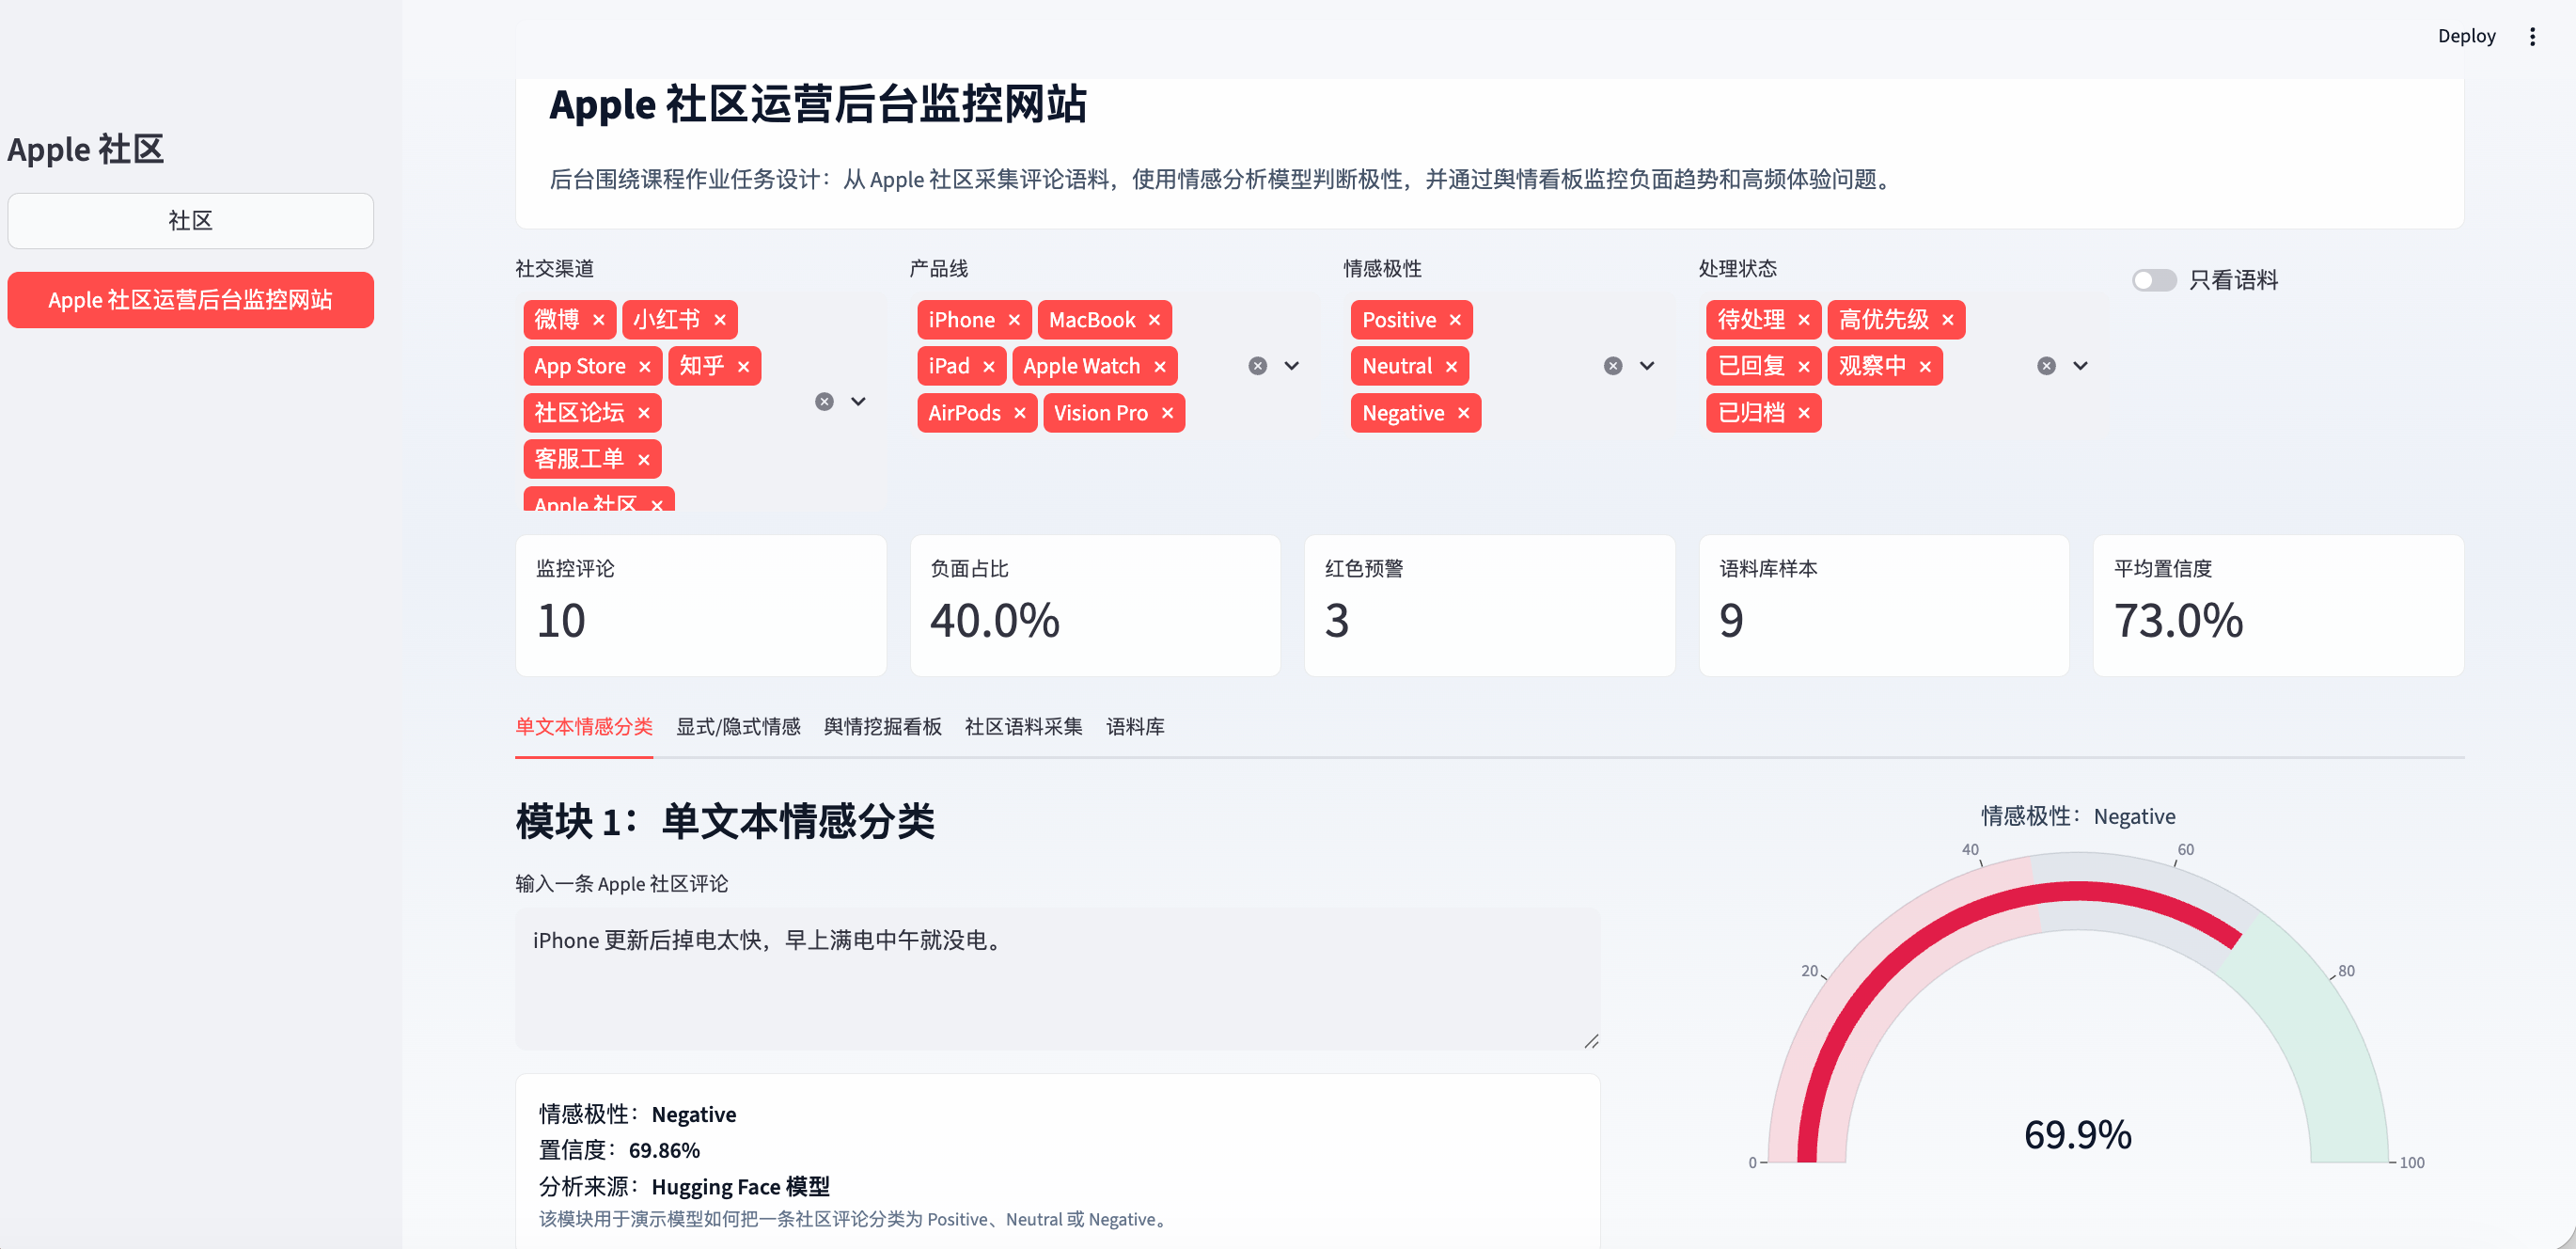
\includegraphics[width=0.6\textwidth]{./picture/module_1.png}
  \caption{模块一界面示例：输入评论后，系统输出情感标签和置信度。}
  \label{fig:example}
\end{figure}


\subsection*{功能说明}

该模块用于对单条 Apple 社区评论进行情感极性分析。用户输入一条评论后，
系统输出情感标签、模型置信度以及仪表盘展示结果。

\begin{itemize}
  \item \textbf{输入：} 一条社区评论，例如 ``AirPods 降噪很好，地铁通勤舒服多了''。
  \item \textbf{输出：} Positive、Neutral 或 Negative。
  \item \textbf{辅助指标：} 置信度，用于衡量模型对当前判断的把握程度。
\end{itemize}

\subsection*{为什么需要置信度}

在真实工程应用中，分类结果通常不能单独作为自动决策依据。
同样被判定为 Negative 的评论，置信度为 95\% 和 58\% 的处理方式应该不同。

\begin{center}
\begin{tabular}{>{\raggedright\arraybackslash}p{3.2cm} >{\raggedright\arraybackslash}p{4.2cm} >{\raggedright\arraybackslash}p{5.6cm}}
\toprule
\textbf{置信度区间} & \textbf{系统动作} & \textbf{原因} \\
\midrule
高置信度 & 自动入库、触发预警或分派工单 & 模型判断稳定，可支撑自动化流程。 \\
中等置信度 & 标记为待确认 & 需要结合关键词、产品线和上下文再次判断。 \\
低置信度 & 进入人工复核队列 & 可能存在反讽、错别字、新梗或模型未见过的表达。 \\
\bottomrule
\end{tabular}
\end{center}

\section*{二、模块二：显式情感与隐式情感识别}

\taskbox{二、观察任务：}{
分别输入一句显式负面评价（如“这屏幕画质太垃圾了”）和一句隐式负面评价
（如“在太阳底下根本看不清屏幕上的字”）。观察现有的小型深度学习模型能否
准确“听懂”隐式表达背后的负面态度。
}

\begin{figure}[htbp]
  \centering
  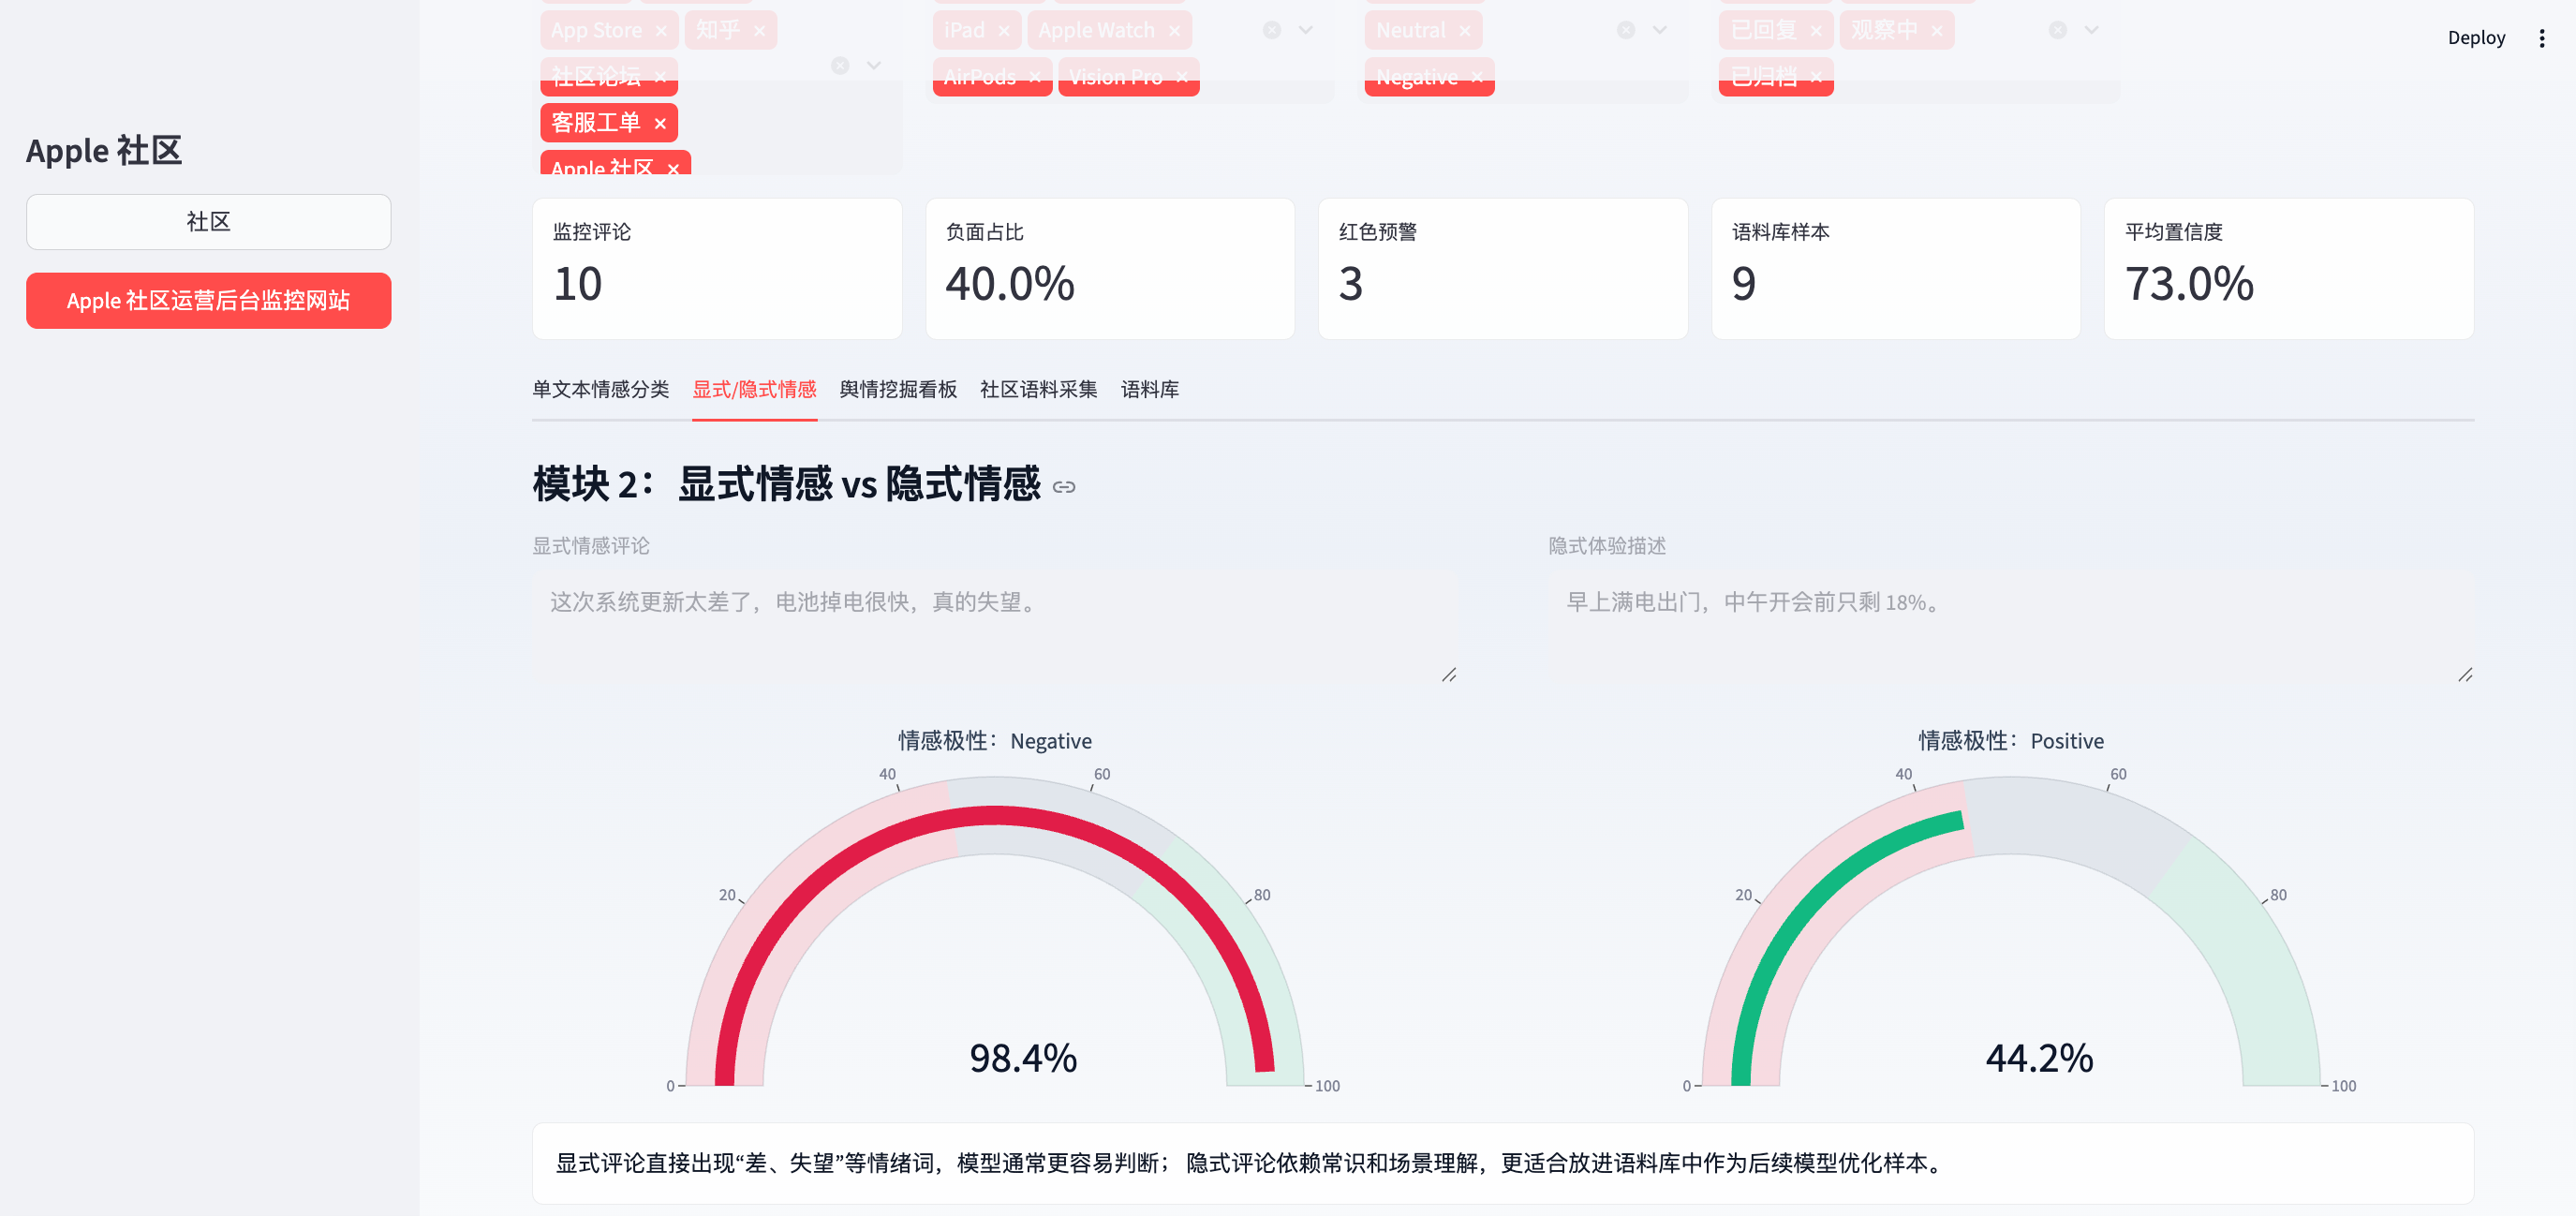
\includegraphics[width=0.6\textwidth]{./picture/module_2.png}
  \caption{模块二界面示例：输入显式和隐式负面评论，观察模型的识别结果。}
  \label{fig:example}
\end{figure}

\subsection*{功能说明}

该模块比较两类评论的识别难度：

\begin{itemize}
  \item \textbf{显式情感：} 直接包含褒贬词，例如 ``垃圾''、``失望''、``很好''。
  \item \textbf{隐式情感：} 表面上是事实描述，但背后包含态度，例如 ``阳光下看不清屏幕''。
\end{itemize}

\subsection*{模型观察重点}

小型深度学习模型通常更容易识别显式情感，因为关键词和训练样本中的模式较明显。
隐式情感则需要模型具备一定的常识推理能力：它要知道 ``看不清屏幕'' 对手机或平板体验来说是负面问题。

如果模型无法稳定识别隐式负面评论，说明后续工程中需要：

\begin{enumerate}
  \item 补充更多真实社区语料，尤其是隐式表达、反讽表达和场景化描述。
  \item 建立人工标注流程，把低置信度样本沉淀为训练集。
  \item 针对 Apple 产品场景建立领域词表，例如续航、发热、断连、屏幕亮度等。
\end{enumerate}

\section*{三、模块三：批量分析、意见挖掘与宏观监控}

\taskbox{三、观察任务：}{
点击批量分析后，观察宏观图表的生成过程。体会将单句的情感分析技术扩展到
大规模语料库时（意见挖掘），是如何为商业决策（如产品改进、危机预警）
提供宏观洞察的。
}

\begin{figure}[htbp]
  \centering
  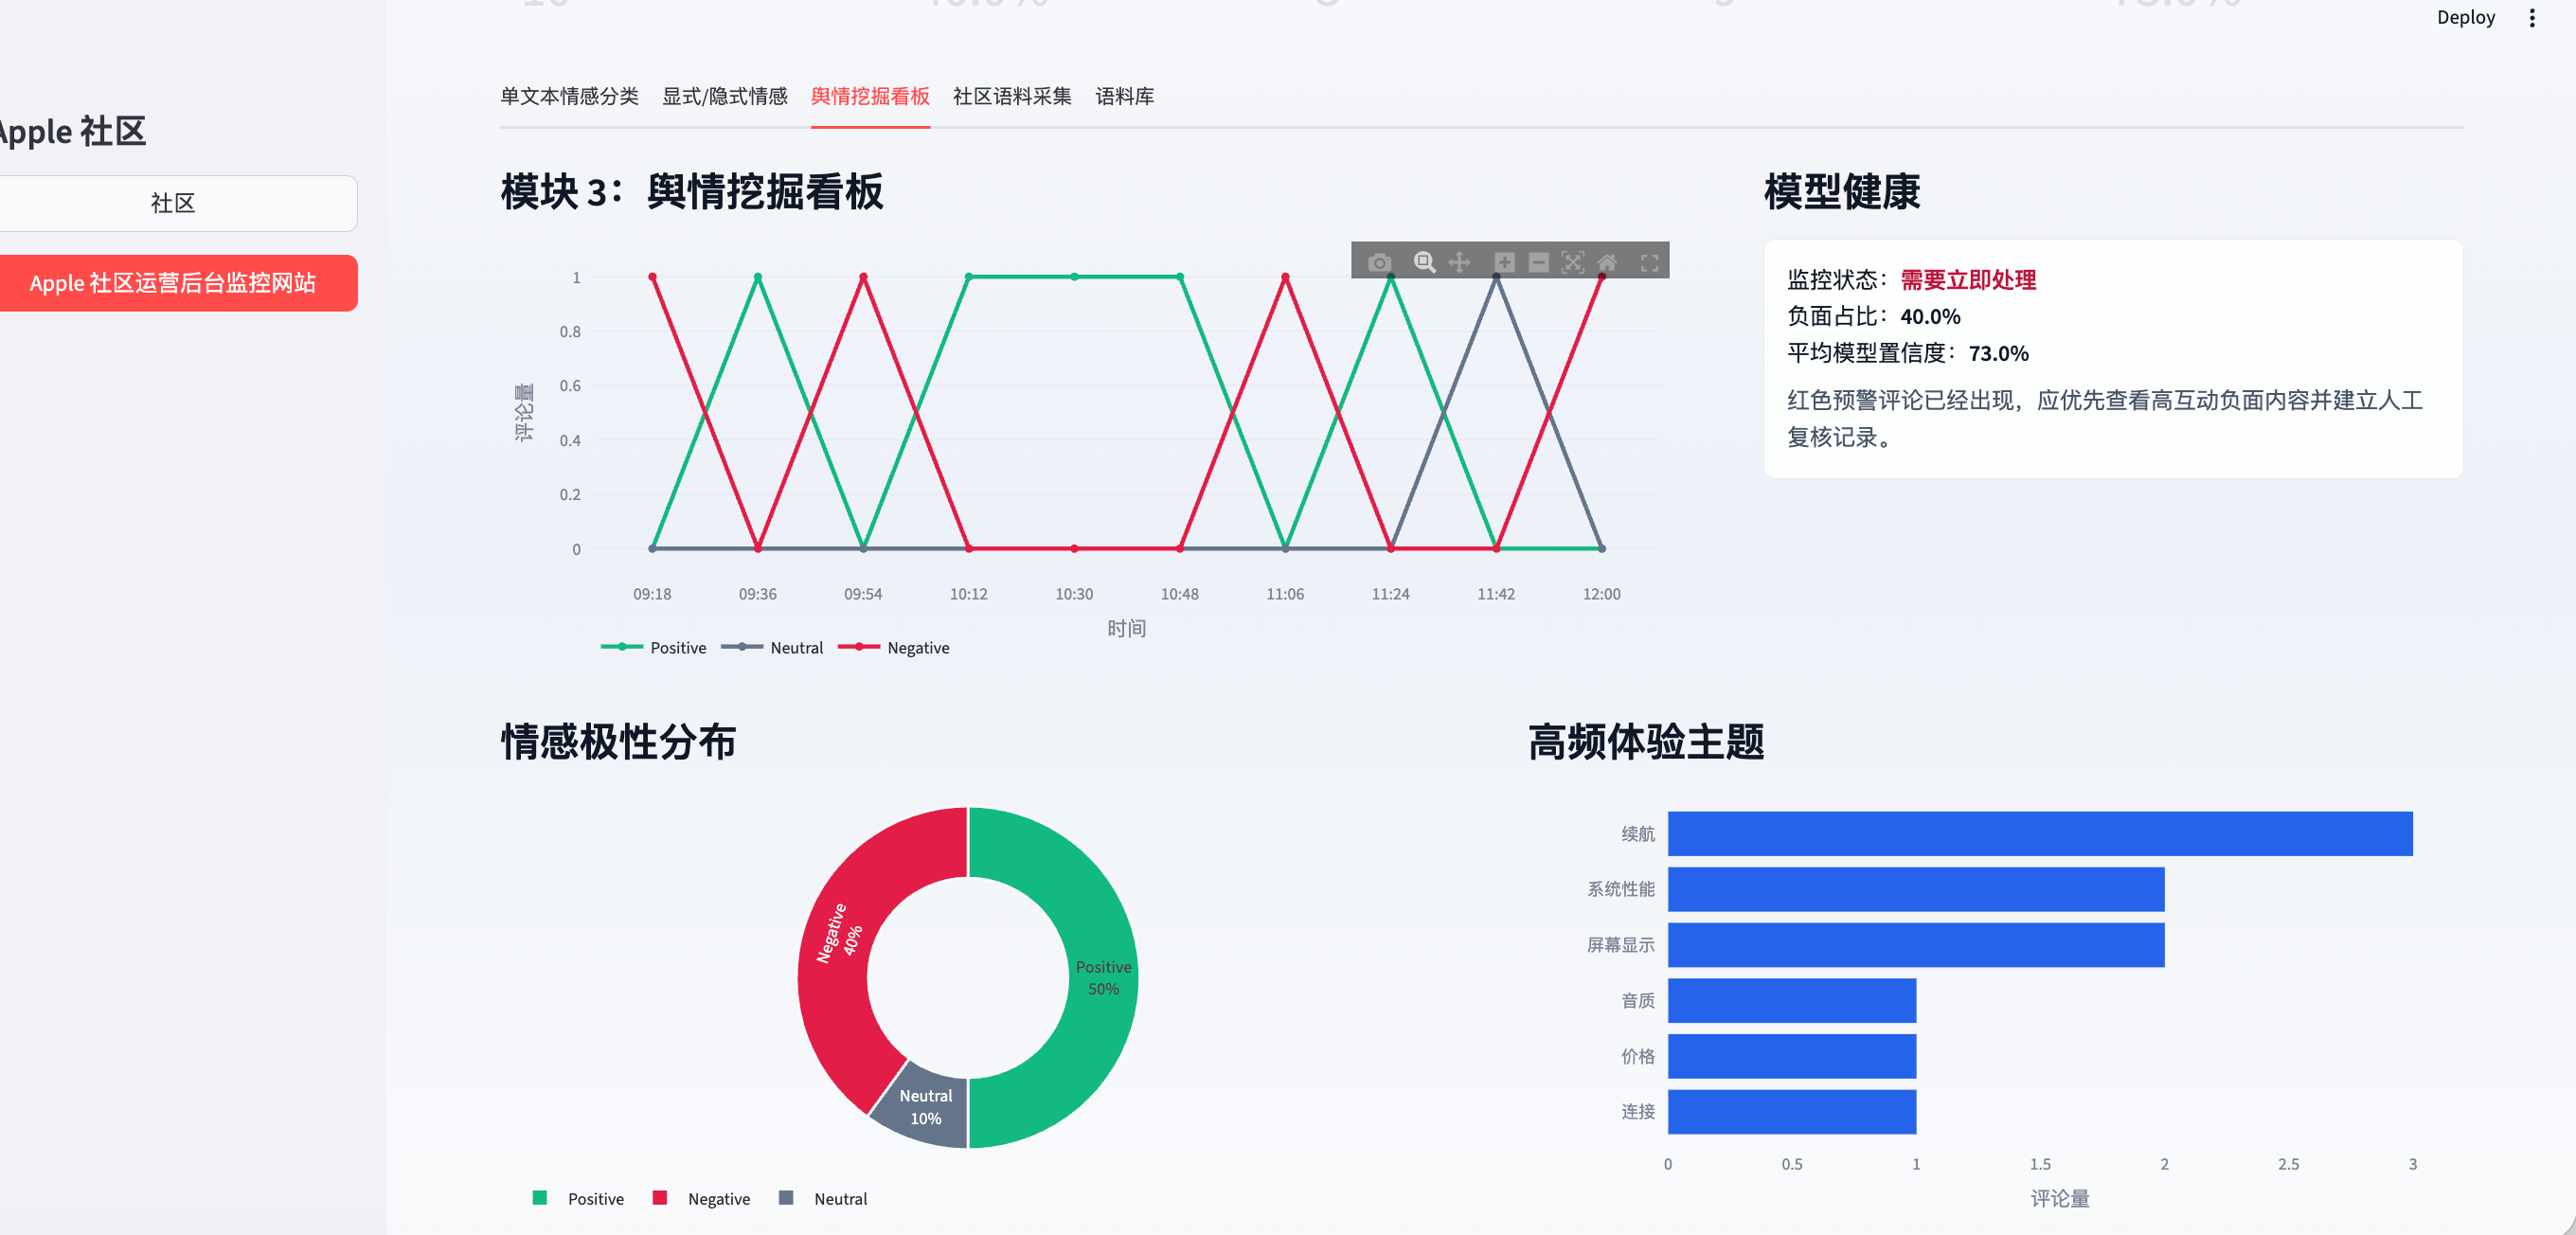
\includegraphics[width=0.6\textwidth]{./picture/module_3.png}
  \caption{模块三界面示例：输入批量评论后，系统输出情感标签和置信度。}
  \label{fig:example}
\end{figure}

\subsection*{功能说明}

该模块将单句情感分析扩展为批量语料分析。系统从 Apple 社区、社交媒体和客服工单中采集评论，
对每条评论进行极性判断，并生成舆情看板。

\begin{itemize}
  \item \textbf{情感分布图：} 展示 Positive、Neutral、Negative 的总体占比。
  \item \textbf{趋势图：} 观察负面评论是否在某个时间段集中升高。
  \item \textbf{主题统计：} 统计续航、发热、屏幕、连接、服务等高频问题。
  \item \textbf{风险预警：} 对高互动、高置信度负面评论进行重点提示。
\end{itemize}

\subsection*{商业决策价值}

当系统发现 ``续航'' 和 ``发热'' 相关负面评论持续上升时，产品团队可以优先排查系统更新、
硬件温控或电池策略问题。当某条负面评论互动量很高时，运营团队可以提前介入，
避免问题扩散为舆情危机。相反，高置信度正面评论可以沉淀为产品卖点，用于内容运营和用户案例整理。

\section*{四、工程落地常见问题}

\subsection*{1. 模型准确率与业务风险不一致}

离线测试准确率较高，不代表线上业务风险低。真实社区中会出现错别字、缩写、新梗、
反讽和多产品混合评价。工程系统应保留置信度、人工复核和错误样本回流机制。

\subsection*{2. 语料采集需要合规与去噪}

社区语料可能包含个人信息、无关广告、重复评论和情绪宣泄。落地时需要进行脱敏、
去重、垃圾文本过滤，并明确数据使用范围。

\subsection*{3. 类别不均衡会影响监控判断}

真实业务中负面评论数量可能远少于中性评论，但负面评论的业务价值更高。
训练和评估时不能只看总体准确率，还应关注负面召回率、误报率和高风险样本覆盖率。

\subsection*{4. 隐式表达和领域知识难以泛化}

``在太阳底下看不清屏幕''、``开会半小时就烫手'' 等评论需要产品场景知识。
通用模型可能无法准确理解，需要结合领域词表、人工标注和持续微调。

\subsection*{5. 看板指标需要可解释}

运营人员不仅需要知道负面比例升高，还需要知道问题集中在哪些产品、哪些主题、
哪些渠道。只有可解释的统计维度，才能真正支持产品改进和危机预警。

\section*{总结}

三个模块共同构成一个从 ``社区语料采集'' 到 ``单句情感识别'' 再到 ``大规模舆情监控''
的完整流程。单文本分类解决微观判断问题，显式/隐式对比帮助理解模型能力边界，
批量意见挖掘则把 NLP 技术转化为可服务运营和产品决策的宏观洞察。

\end{document}
